\documentclass{beamer}
\usetheme{Singapore}
\usepackage[round,sort]{natbib}
\usepackage{tikz}
\usetikzlibrary{arrows,decorations.pathmorphing,backgrounds,fit,positioning,shapes.symbols,chains}
\usepackage{adjustbox}
\usepackage{verbatim}
\usepackage{graphicx}
\graphicspath{ {etig-05-aiyenggar-images/} }

\title{Diffusion of Innovation}
\subtitle{A Review of Readings}
\author{Ashwin Iyenggar}
\institute[Indian Institute of Management Bangalore] 
{
  Corporate Strategy and Policy\\
  Indian Institute of Management Bangalore
}
\date{28 January, 2017}
\subject{Review of Assigned Readings on bridging the macro \& and micro aspects of innovation}

% \pgfdeclareimage[height=0.5cm]{university-logo}{university-logo-filename}
% \logo{\pgfuseimage{university-logo}}

\AtBeginSubsection[]
{
  \begin{frame}<beamer>{Outline}
    \tableofcontents[currentsection,currentsubsection]
  \end{frame}
}

\begin{document}

\begin{frame}
  \titlepage
\end{frame}

\begin{frame}{Outline}
  \tableofcontents
  % You might wish to add the option [pausesections]
\end{frame}

\section{Overview}
\begin{frame}{Bridging the micro and macro aspects of Innovation}{}
\begin{itemize}
\item{General Purpose Technologies and Innovation}
\item{Diffusion of Innovation}
\item{Trade and Innovation}
\end{itemize}
\end{frame}

\begin{frame}{Diffusion of Innovation}{}
\begin{itemize}
\item{\cite{Stoneman2010} - Technological diffusion from demand and supply side, at different levels of analysis}
\item{\cite{Atkin2015} - Empirical study on organizational impediments to adoption of technology}
\item{\cite{Bollinger2012} - Empirical study of peer effects in technology diffusion}
\end{itemize}
\end{frame}






\section{\cite{Stoneman2010}}
\begin{frame}{The Diffusion of New Technology}{Agenda}
\begin{itemize}
\item{Scope of Definition of Technology Diffusion}
\item{Demand and Supply Side}
\item{Diffusion at different levels of aggregation - worldwide, industry, household}
\end{itemize}
\end{frame}


\begin{frame}{The Diffusion of New Technology}{Prior Literature}
\begin{itemize}
\item{Tended to confine analysis of diffusion to the study of the use of new technology by firms for the first time, or household demands for new products - A blinkered view?}
\item{\cite{Stoneman2010} Definition: Process by which the market for a new technology changes over time and from which ownership or usage patterns result}
\item{Advantage 1: Market implies both sides: supply and demand}
\item{Advantage 2: Definition of term market does not imply spatial boundaries}
\item{International diffusion literature conflates intensive (within country) and extensive (across countries)}
\item{Supply side is less studied in diffusion studies}
\item{Supply can include imports, Demand can include exports}
\end{itemize}
\end{frame}

\begin{frame}{The Diffusion of New Technology}{International Patterns in use of new technologies}
\begin{itemize}
\item{Cross-country dispersion in technology adoption is 3-5x larger than cross-country dispersion in income per capita}
\item{High correlation in relative position of countries' degree of technological adoption across technologies}
\item{Convergence within technologies at 4-7\% a year}
\item{Speed of convergence after 1925 is 3x that of technologies developed before 1925}
Source: Comin et al. (2006)
\end{itemize}
\end{frame}

\begin{frame}{The Diffusion of New Technology}{International Patterns in Production}
\begin{figure}[h]
\begin{centering}
  \includegraphics[width=\textwidth]{stoneman1}
  \caption{Source: \cite{Stoneman2010}}
   \label{fig:stoneman1}
\end{centering}
\end{figure}
\end{frame}

\begin{frame}{The Diffusion of New Technology}{National Contexts}
\begin{itemize}
\item{Klepper and Graddy (1990)  three stages: a) initial stage with large and growing number of producers, b) shakeout, and c) number of producers stabilizes}
\item{Klepper and Graddy (1990) - industries start with very fast rates of growth which then decline with maturity}
\item{No reason why the firms that exist in an industry at a late stage have to enter ab initio}
\item{Due to exports, production patterns do not match completely with the concept of supply to a national product market}
\item{The example of the US may not be typical for all countries}
\item{Patent system may well constrain entry to new industries}
\end{itemize}
\end{frame}

\begin{frame}{The Diffusion of New Technology}{Industries, Firms, Households}
\begin{itemize}
\item{S sharped curve at international, national, industrial, and firm levels whereby usage increases slowly and then accelerates up to a point of inflection after which usage continues to grow but at a declining rate until the asymptote is reached}
\item{Comparisons are not simple: three parameters of concern - local date of first use, asymptotic level of use, speed of diffusion}
\item{Diffusion paths may differ across technologies}
\item{Early and late adopters have different characteristics}
\end{itemize}
\end{frame}

\begin{frame}{The Diffusion of New Technology}{Demand Side Modeling}
\begin{itemize}
\item{Disequilibrium models: passive learning, and evolutionary economics}
\item{Equilibrium models: all moments in time, markets clear, and firms and households are rational and are driven by profit and utility maximization respectively}
\item{label order effects - are there first mover advantages that lead to firms competing to be an early adopter?}
\item{Cost of acquiring new technology - diffusion driven by exogenous changes in cost}
\item{Alternate strategies: predation and preemption - building on game theory/Nash equilibrium}
\item{Uncertainty - search models, passive information acquisition models, strategic information models: Are reductions in uncertainty self-perpetuating?}

\end{itemize}
\end{frame}

\begin{frame}{The Diffusion of New Technology}{Supply Side Modeling}
\begin{itemize}
\item{The cost structure of the supplying industry}
\item{The market structure of the supplying industry}
\item{Incentives to provide product information to buyers}
\item{Internationalized supply side industries - learning by doing, scale economies, incentives to R\&D and international arbitrate may all affect the rate of diffusion in far off markets}
\end{itemize}
\end{frame}

\begin{frame}{The Diffusion of New Technology}{Issues}
\begin{itemize}
\item{Is diffusion self-propagating or does it require continuous outside stimuli?}
\item{What are the appropriate levels of aggregation at which to analyze diffusion?}
\end{itemize}
\end{frame}

\begin{frame}{The Diffusion of New Technology}{Factors}
\begin{figure}[h]
\begin{centering}
  \includegraphics[width=\textwidth]{stoneman2}
  \caption{Source: \cite{Stoneman2010}}
   \label{fig:stoneman2}
\end{centering}
\end{figure}
\end{frame}

\begin{frame}{The Diffusion of New Technology}{Factors}
\begin{itemize}
\item{A basic problem in diffusion policy is in deciding what is a desirable outcome}
\item{Heterogeneity in: capital requirements, labor requirements, time lag, and uncontrollable aspects of technology}
\item{Diffusion process in interfirm and intrafirm literatures highlight the following (for producer technology}
\item{firms of different characteristics obtain different returns from using or extending usage of new technology - rank effects}
\item{there are market intermediated stock and/or order effects}
\item{nonmarket intermediated spillovers to other users}
\item{intrafirm usage lages interfirm usage}
\end{itemize}
\end{frame}



\section{\cite{Atkin2015}}
\begin{frame}{Organizational Barriers to Technology Adoption}{Summary}
\begin{itemize}
\item{Firms take long to adapt to new technology}
\item{Misalignment of incentives may be a major barrier in technological adoption}
\end{itemize}
\end{frame}

\begin{frame}{Organizational Barriers to Technology Adoption}{Methodology}
\begin{itemize}
\item{135 firms, Randomly allocated new technology to 35 firms ("tech drop")}
\item{18 firms given cash equivalent to new die ("cash drop")}
\item{79 firms were given nothing ("no drop")}
\item{After 15 months, five frims from tech-drop group and one from the no-drop group had used the new die to produce more than 1000 balls}
\item{Survey in March-April 2013 to find out reasons for non-adoption}
\item{Incentive-Payment experiment September-November 2013 on 35 tech drop firms}
\end{itemize}
\end{frame}

\begin{frame}{Organizational Barriers to Technology Adoption}{Summary}
\begin{figure}[h]
\begin{centering}
  \includegraphics[width=\textwidth]{atkin1}
  \caption{Source: \cite{Atkin2015}}
   \label{fig:atkin1}
\end{centering}
\end{figure}
\end{frame}

\begin{frame}{Organizational Barriers to Technology Adoption}{Summary}
\begin{figure}[h]
\begin{centering}
  \includegraphics[width=\textwidth]{atkin2}
  \caption{Source: \cite{Atkin2015}}
   \label{fig:atkin2}
\end{centering}
\end{figure}
\end{frame}

\begin{frame}{Organizational Barriers to Technology Adoption}{Summary}
\begin{figure}[h]
\begin{centering}
  \includegraphics[width=\textwidth]{atkin3}
  \caption{Source: \cite{Atkin2015}}
   \label{fig:atkin3}
\end{centering}
\end{figure}
\end{frame}

\begin{frame}{Organizational Barriers to Technology Adoption}{Summary}
\begin{figure}[h]
\begin{centering}
  \includegraphics[width=\textwidth]{atkin4}
  \caption{Source: \cite{Atkin2015}}
   \label{fig:atkin4}
\end{centering}
\end{figure}
\end{frame}

\begin{frame}{Organizational Barriers to Technology Adoption}{Summary}
\begin{figure}[h]
\begin{centering}
  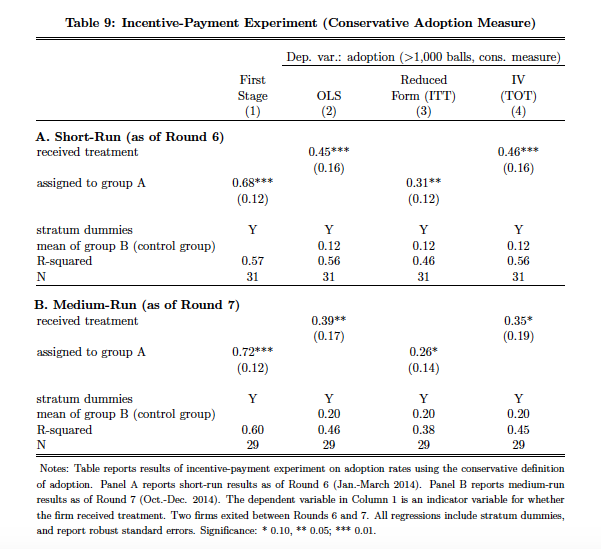
\includegraphics[width=\textwidth]{atkin5}
  \caption{Source: \cite{Atkin2015}}
   \label{fig:atkin5}
\end{centering}
\end{figure}
\end{frame}

\begin{frame}{Organizational Barriers to Technology Adoption}{Summary}
\begin{figure}[h]
\begin{centering}
  \includegraphics[width=\textwidth]{atkin6}
  \caption{Source: \cite{Atkin2015}}
   \label{fig:atkin6}
\end{centering}
\end{figure}
\end{frame}

\begin{frame}{Organizational Barriers to Technology Adoption}{Summary}
\begin{figure}[h]
\begin{centering}
  \includegraphics[width=\textwidth]{atkin7}
  \caption{Source: \cite{Atkin2015}}
   \label{fig:atkin7}
\end{centering}
\end{figure}
\end{frame}

\begin{frame}{Organizational Barriers to Technology Adoption}{Extension}
\begin{itemize}
\item{The industry studied produces a standardized product. The results may therefore be endogenous to the industry stage of maturity}
\item{In highly innovative industries, one would expect different dynamics at work}
\end{itemize}
\end{frame}


\section{\cite{Bollinger2012}}
\begin{frame}{Peer Effects in Technology Diffusion}{Summary}
\begin{itemize}
\item{Is there a causal social interaction effect for the social spillovers to exist?}
\item{The canonical Bass (1969) model assumes social contagion to be a driving force behind accelerating adoption rates}
\item{This article documents and estimates the magnitude of peer effects in diffusion of solar photovoltaic panels}
\item{Issues in indentification of peer effects: endogenous group formation leading to self-selection of peers, correlated unobservables, and simultaneity}
\item{Using daily adoption data, leveraging a DiD to avoid functional or distributional assumptions on the data generating process, controlling for endogeneity, and avoiding the fixed effects biases}
\end{itemize}
\end{frame}

\begin{frame}{Peer Effects in Technology Diffusion}{Method}
\begin{itemize}
\item{Leverage the fact that in solar PV market, the decision  to install solar panels does not lead to an instantaneous installation due to time needed for paper work and installation}
\item{Do not expect social interactions to have an effect until the solar PV panels have actually been installed}
\item{Analysis at the zipcode level}
\item{Several estimation methods used: traditional fixed effects estimation taking mean differences on the zip code-quarter, zip-quarter random effects, first differences  (preferred)}
\item{Using daily adoption data, leveraging a DiD to avoid functional or distributional assumptions on the data generating process, controlling for endogeneity, and avoiding the fixed effects biases}
\end{itemize}
\end{frame}

\begin{frame}{Peer Effects in Technology Diffusion}{Results}
\begin{figure}[h]
\begin{centering}
  \includegraphics[width=\textwidth]{bollinger1}
  \caption{Source: \cite{Bollinger2012}}
   \label{fig:bollinger1}
\end{centering}
\end{figure}
\end{frame}

\bibliography{/Users/aiyenggar/OneDrive/code/bibliography/ae,/Users/aiyenggar/OneDrive/code/bibliography/fj,/Users/aiyenggar/OneDrive/code/bibliography/ko,/Users/aiyenggar/OneDrive/code/bibliography/pt,/Users/aiyenggar/OneDrive/code/bibliography/uz}
\bibliographystyle{apalike}

\end{document}

\begin{comment}
\begin{figure}[h]
\begin{centering}
  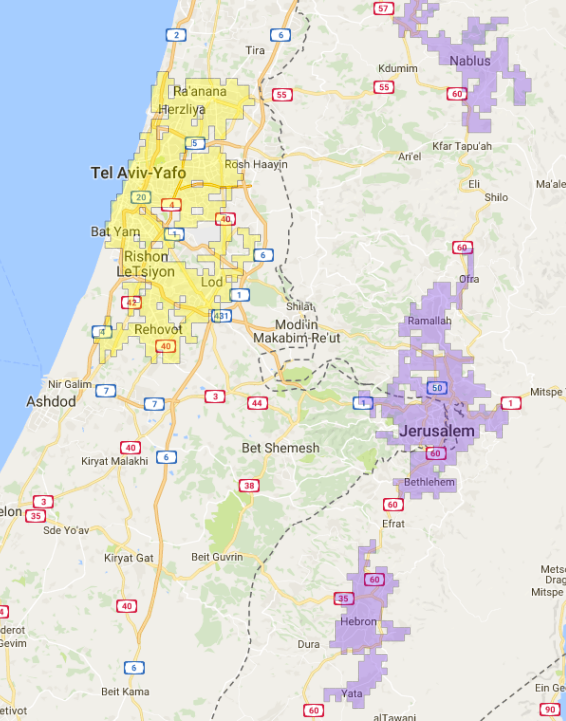
\includegraphics[width=\textwidth]{TelAviv}
  \caption{Geographic Definition of Tel Aviv-Yafo}
   \label{fig:TelAviv}
\end{centering}
\end{figure}
\end{comment}

